\documentclass[main.tex]{subfiles}

\begin{document}

\chapter{Post Assembly} \label{chapter:postassembly}

In previous part we saw several third generation assembly tools, each on have their own specificity and method to produce a long read assembly. Each assembly tools produce different output files, but all of them produce a contigs file that store contigs sequences build during assembly. Other files generally contains information about contigs, coverage, if a contigs is circular or not, which reads is included to which contigs, ….

All this information is useful to assess the assembly quality, or to integrate other information to improve the assembly. In this chapter we will briefly review some methods for evaluating an assembly and will especially focus on the most commonly used method for evaluating a new assembly. 
The alignment of the contigs of the assembly against a known reference.%PHRASE NOMINALE=DANGER
We will see that this method requires some adjustment when evaluating an uncorrected assembly pipeline.

In a second part we  observe how recent assembly long-read assembly tools still failed to produce a good assembly on data where  it should  theoretically succeed. We thereafter present our solution \knot. \knot is a tool which by returning to the original information reads, tries to find information that could not be used by the assembly pipelines.%GNU ?


\section{Assembly evaluation} 

Several metrics exist to compare and evaluate assembly. The most common metric used is the N50 that evaluate the contiguity of assembly. For example we take a genome with one chromosomes and two assembly. The first assembly contains one large contigs (approximately the length of chromosomes) and many short. The second contains only contigs of average size one or two order of magnitude smaller than the chromosomes. The first one have an higher contiguity we have more information about the genome with the first assembly than the second we didn't need perform an hard scaffolding step to have an idea of genome organisation.

To compute N50, we create a list of your contigs length and sort them. When the cumulative sum of contigs length (starting with the largest) is larger than the sum of all contigs, the length the last added contig is the N50 value. For example, $L$ is the sorted list of contigs length: 
\begin{equation}
\begin{aligned}
L &= \{20, 30, 40, 50, 70, 80\} \\
L_{sum} &= \sum\limits_{i=0}^{|L|} L_i = 290 \\
\frac{290}{2} &> 20 + 30 + 40 + 50 \\
\frac{290}{2} &< 20 + 30 + 40 + 50 + 70\\
N_{50}(L) &= 70\\
\end{aligned}
\end{equation}

70 was the last length added in cumulative length before this cumulative length is larger than half of the total sum of assembly.
N25, N75 or NX correspond to the same metrics as N50 for 25\%, 75\%, or X\% of total length of contigs. L50 is the rank of the N50 contig in the sorted contigs list, L50 of our example is 5.

NG50 is the same thing as N50, but the total sum of contigs length is replaced by the genome length (estimate or get from a previous assembly). NGA50 is the same as NG50, but the contigs length is replaced by the length of contig that map against the reference genome. We can cite U50 as another metric similar to N50 where overlapping region between contigs was ignored \cite{U50}.

N50 family metrics are not perfect, but they help to represent the contigs length distribution, and to compare the results of different assembly tools on the same dataset. N50 is useful to analyze assembly quality without any external information.

By adding other information, we can evaluate assembly not only on size of contigs. \toolsname{BUSCO}\cite{busco} evaluates the assembly completeness with the presence or the absence of core genes. By mapping contigs against reference genome or close reference genome, \toolsname{Quast}\cite{quast} computes many metrics like the number of misassembly, NGA50, the identity level of contigs, …. 

Some other tools and techniques exist and is useful. Some of them are presented in more details in \cite{seq_assembly_demystified}

\subfile{paper/misassemblies-in-noisy-assemblies.tex}

\section{Trouble with heuristic algorithm}

Assembly tools need to rely on heuristics. Due to theoretical limit, how many of base need to be share between two read to create an overlap, how many error we can accept in this overlap, to memory constraint, computation time limit you can't search and store all overlap.%2 phrases pls
Most of the time chosen heuristics perform  very well, but in some case a more complex analysis is needed.

\citeauthor{long_read_assembler_comparison} in \cite{long_read_assembler_comparison} perform a comparison of five assembly tools on real data and simulated data bacterial data set. Some difficulty is injected in the input long-reads to stress assembly tools:
\begin{itemize}
    \item Adaptor length. Sequencing techniques require the introduction of short sequence before reads. Because of their high error rates to detect and remove those adaptor from long-read sequences is not trivial. Those adaptors can generate  assembly error.
    \item Chimeric read. During DNA extraction and fragmentation, two fragments coming from different regions can be  sequenced as a single read. This can lead to assembly fragmentation.
    \item Glitch level. Long-read error aren't uniformly distributed along the reads and sometimes sequencer create a region with only random sequence. A higher the glitch level indicate a larger region and a higher frequency. 
    \item Random junk reads. Some read are just a string of random character
    \item Read depth, correspond to genome coverage
    \item Read identity, percent of error insertion, deletion, substitution 
    \item Read length
\end{itemize}

\begin{figure}
    \centering
    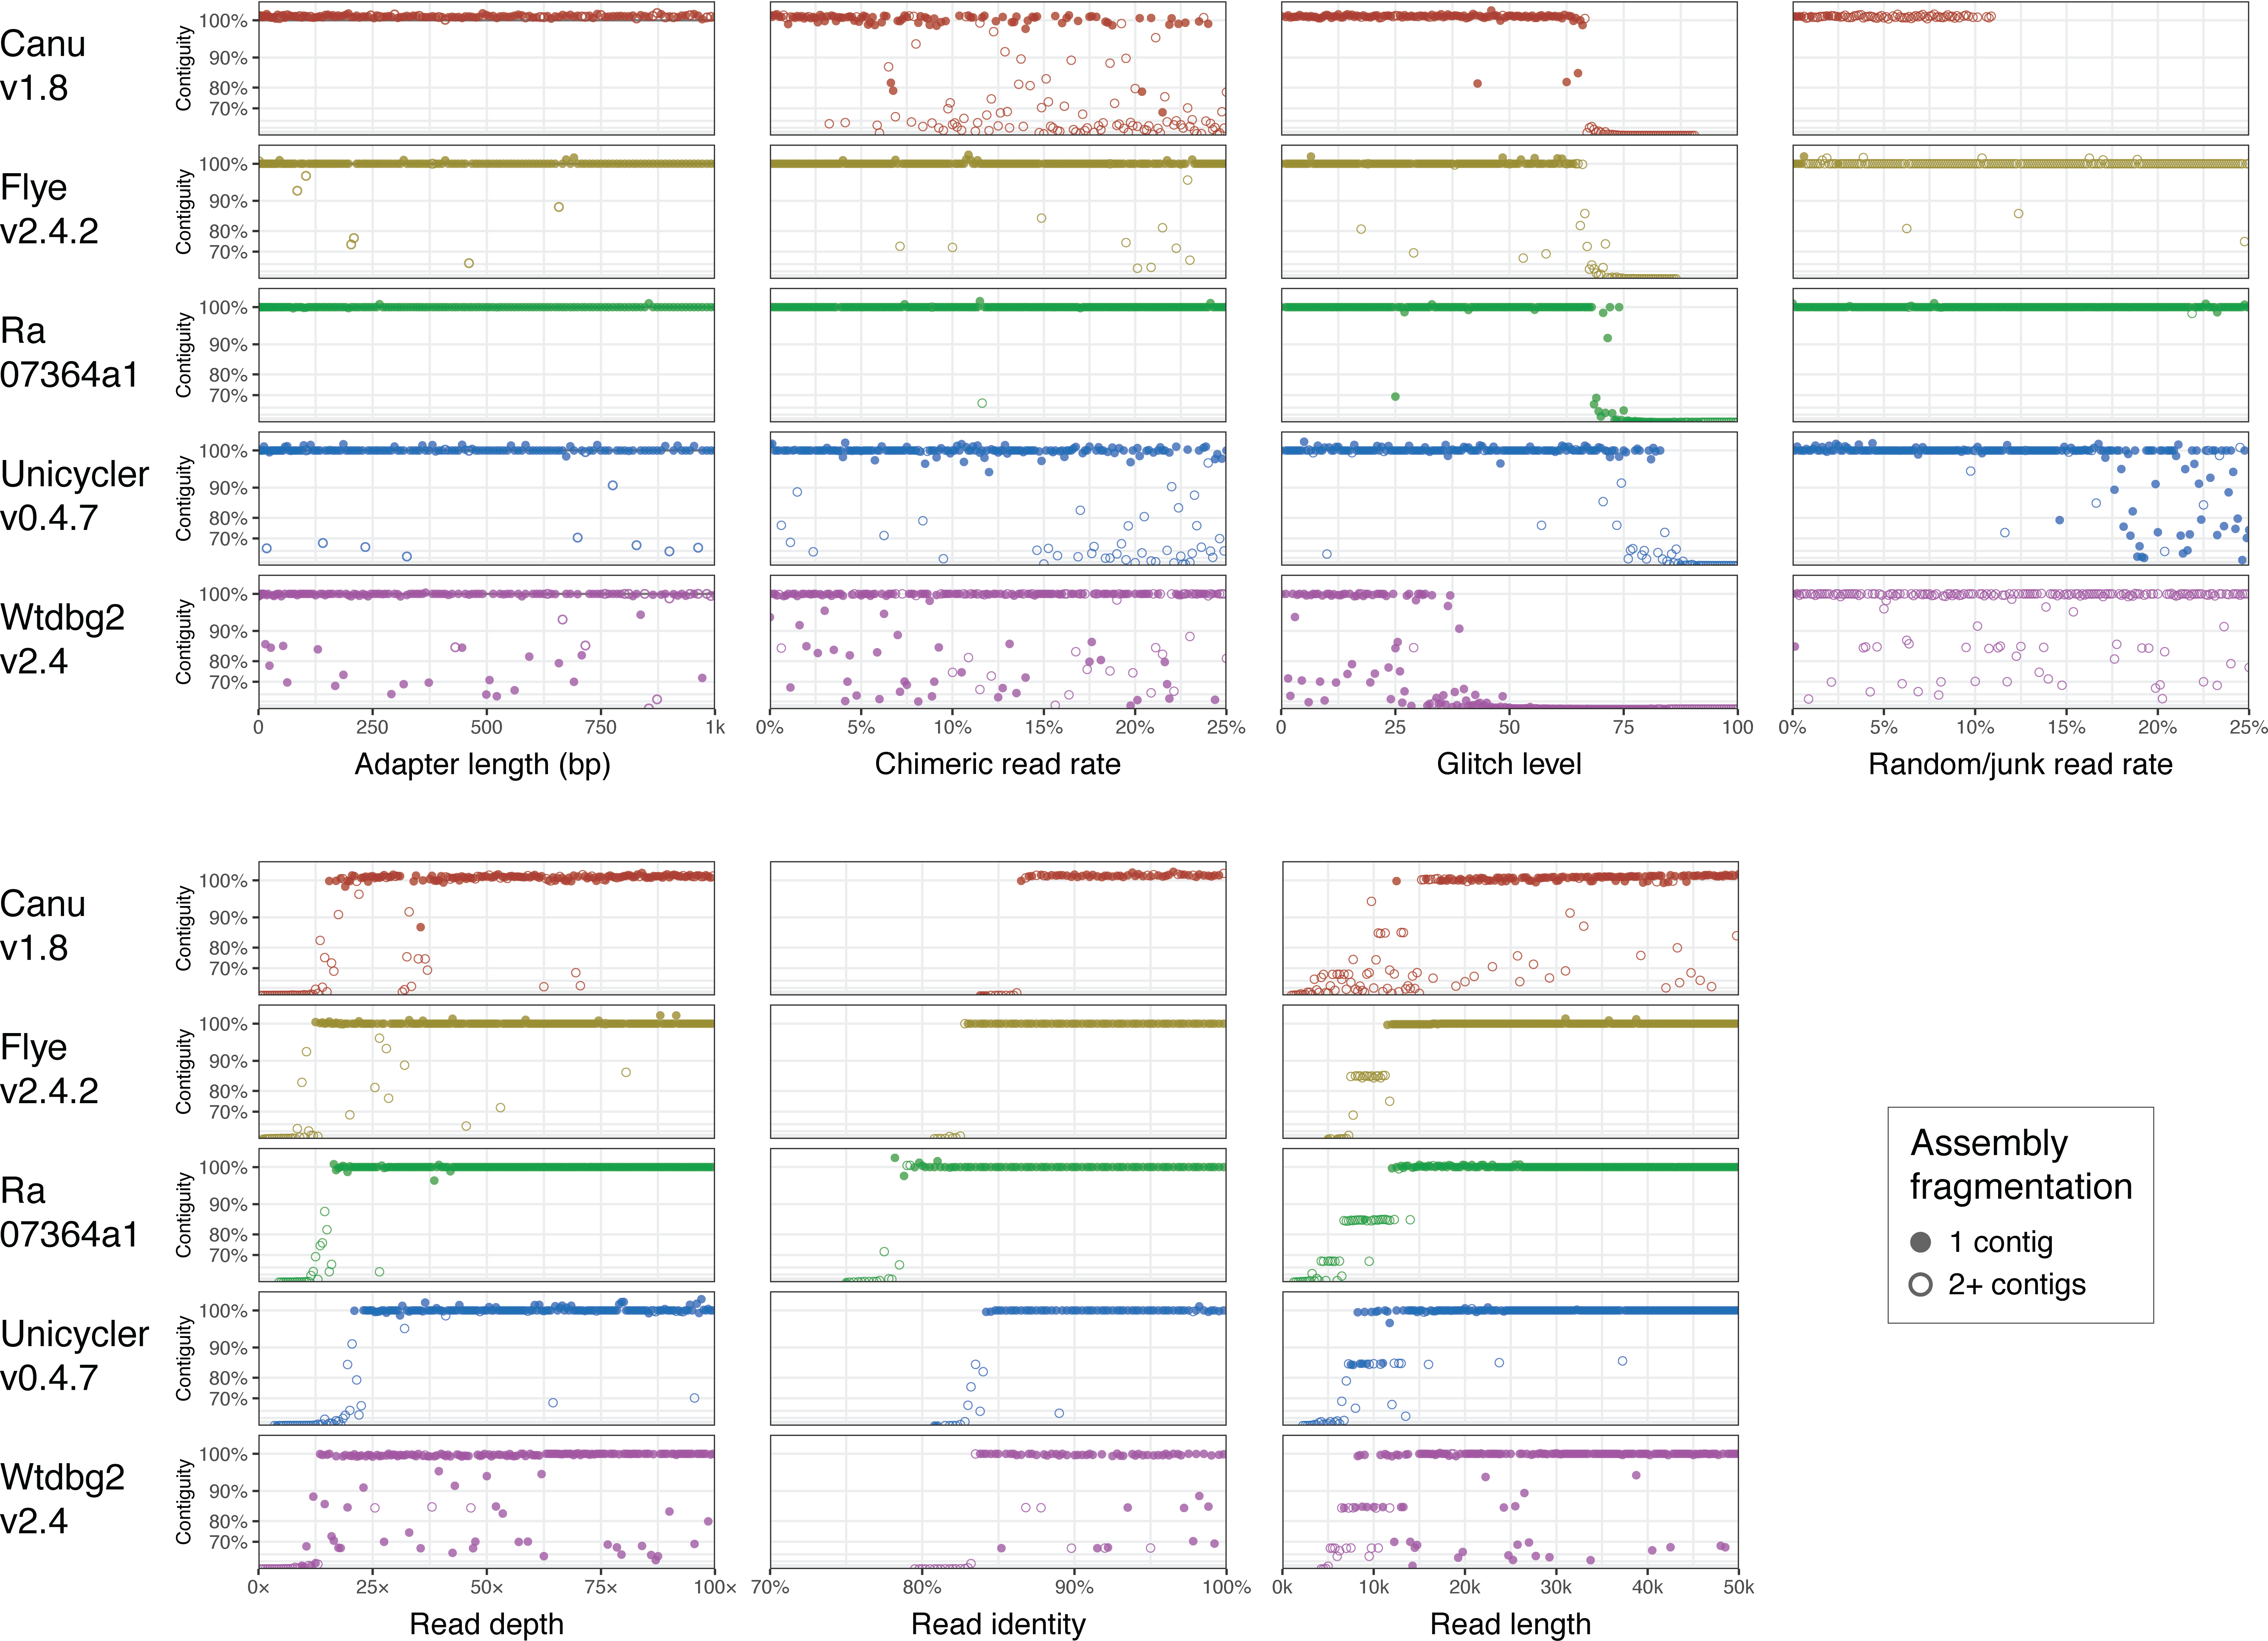
\includegraphics[width=\textwidth]{introduction/images/rrwick_bench.png}
    \caption{Effect of different reads property on assembly contiguity (number of contigs expect and map correctly on reference genome), of five assembly tools. \toolsname{Unicycler} is an hybrid assembler (use second and thrid generation read). \canu is a long-read assembly pipeline they perform a self correction before construct assembly with a special \OLC graph (more detail in Section \ref{section:sota:canu}). \toolsname{Ra} perform a basic string graph assembly on raw reads with a correction of contigs after assembly (more detail in Section \ref{section:sota:miniasm}). \wtdbg and \toolsname{Flye} use a \DBG like approach to perform assembly on raw reads (more detail in Section \ref{section:sota:wtdbg}). This figure is a reproduction of figure from \cite{long_read_assembler_comparison}.}
    \label{intro:fig:rrwick_bench}
\end{figure}

This study focus on  assembly contiguity, if the number of contigs match with the expected number of contig and if  contigs can be mapped against the reference. %Refaire la phrase sans if
All assemblers perform a good assembly when:%according to this benchmarck we observe that
\begin{itemize}
    \item reads length are upper than 10k and lower than 20k, this length can be reach by long-read sequencing technology but requests a particular attention be focused on the risk of DNA fragmentation%MOUAIS
    \item read identity need to be upper than 85\% except %except nadine ?
    \item the minimal coverage is around 20x, but this study didn't analyze the error rate of assembly we can suspect an high error rate in assembled contigs% too soon ?
    \item Chimeric read have an important impact on assembly contiguity but at level generally not observe in real data % ne va pas avec le "when : bla" met "si il n'y a pas bcp de reads chimeric" et discute de tes trucs apres cette liste
\end{itemize}

We can observe an important variability of result (in \canu, \wtdbg and \toolsname{Unicycler}), an assembly can fail for many reason: a chimeric read in a repetition, a drop of coverage, a missing overlap, or a inappropriate  set of parameter.
%UN SAUT TH2MATIQUE DE OUF ICI
We often notice an overlap missed by a given tool but found by another and we observe that overlapping tools on real data have room for progression  \cite{ovl_bench}. 
In section \ref{section:preassembly:ovl_consensus} we talk about difference between overlapping tools result and some preliminary result of an overlapping tools consensus.%GNU

Analysis and understanding of the data produced by assembly tools help to check if assembly result didn't produce false result or to understand, and sometimes solve, assembly trouble. Some tools use remapping of reads against assembled contigs to found misassembly by detect incongruity's in read coverage, mate pairs mapping, read mapping clipping.
Some tools or assembly tools was developed in order to to analyses assembly graph to understand what is happening during assembly like \toolsname{Bandage} \cite{bandage}, a tools to visualize assembly graph.

We developed \knot a tools to simplify analysis of assembly tools result and help users to make choices improving assembly quality.% and found lost link between contigs in assembly. ca va ailleurs ca
This tool is based on the observation that the graph of raw reads is generally connected (we can reach any node from any node), while the graph of contigs does not. Therefore the idea of \knot is to use the graph of raw reads to find the (potentially missed) links between the contigs.

\begin{figure}[ht]
    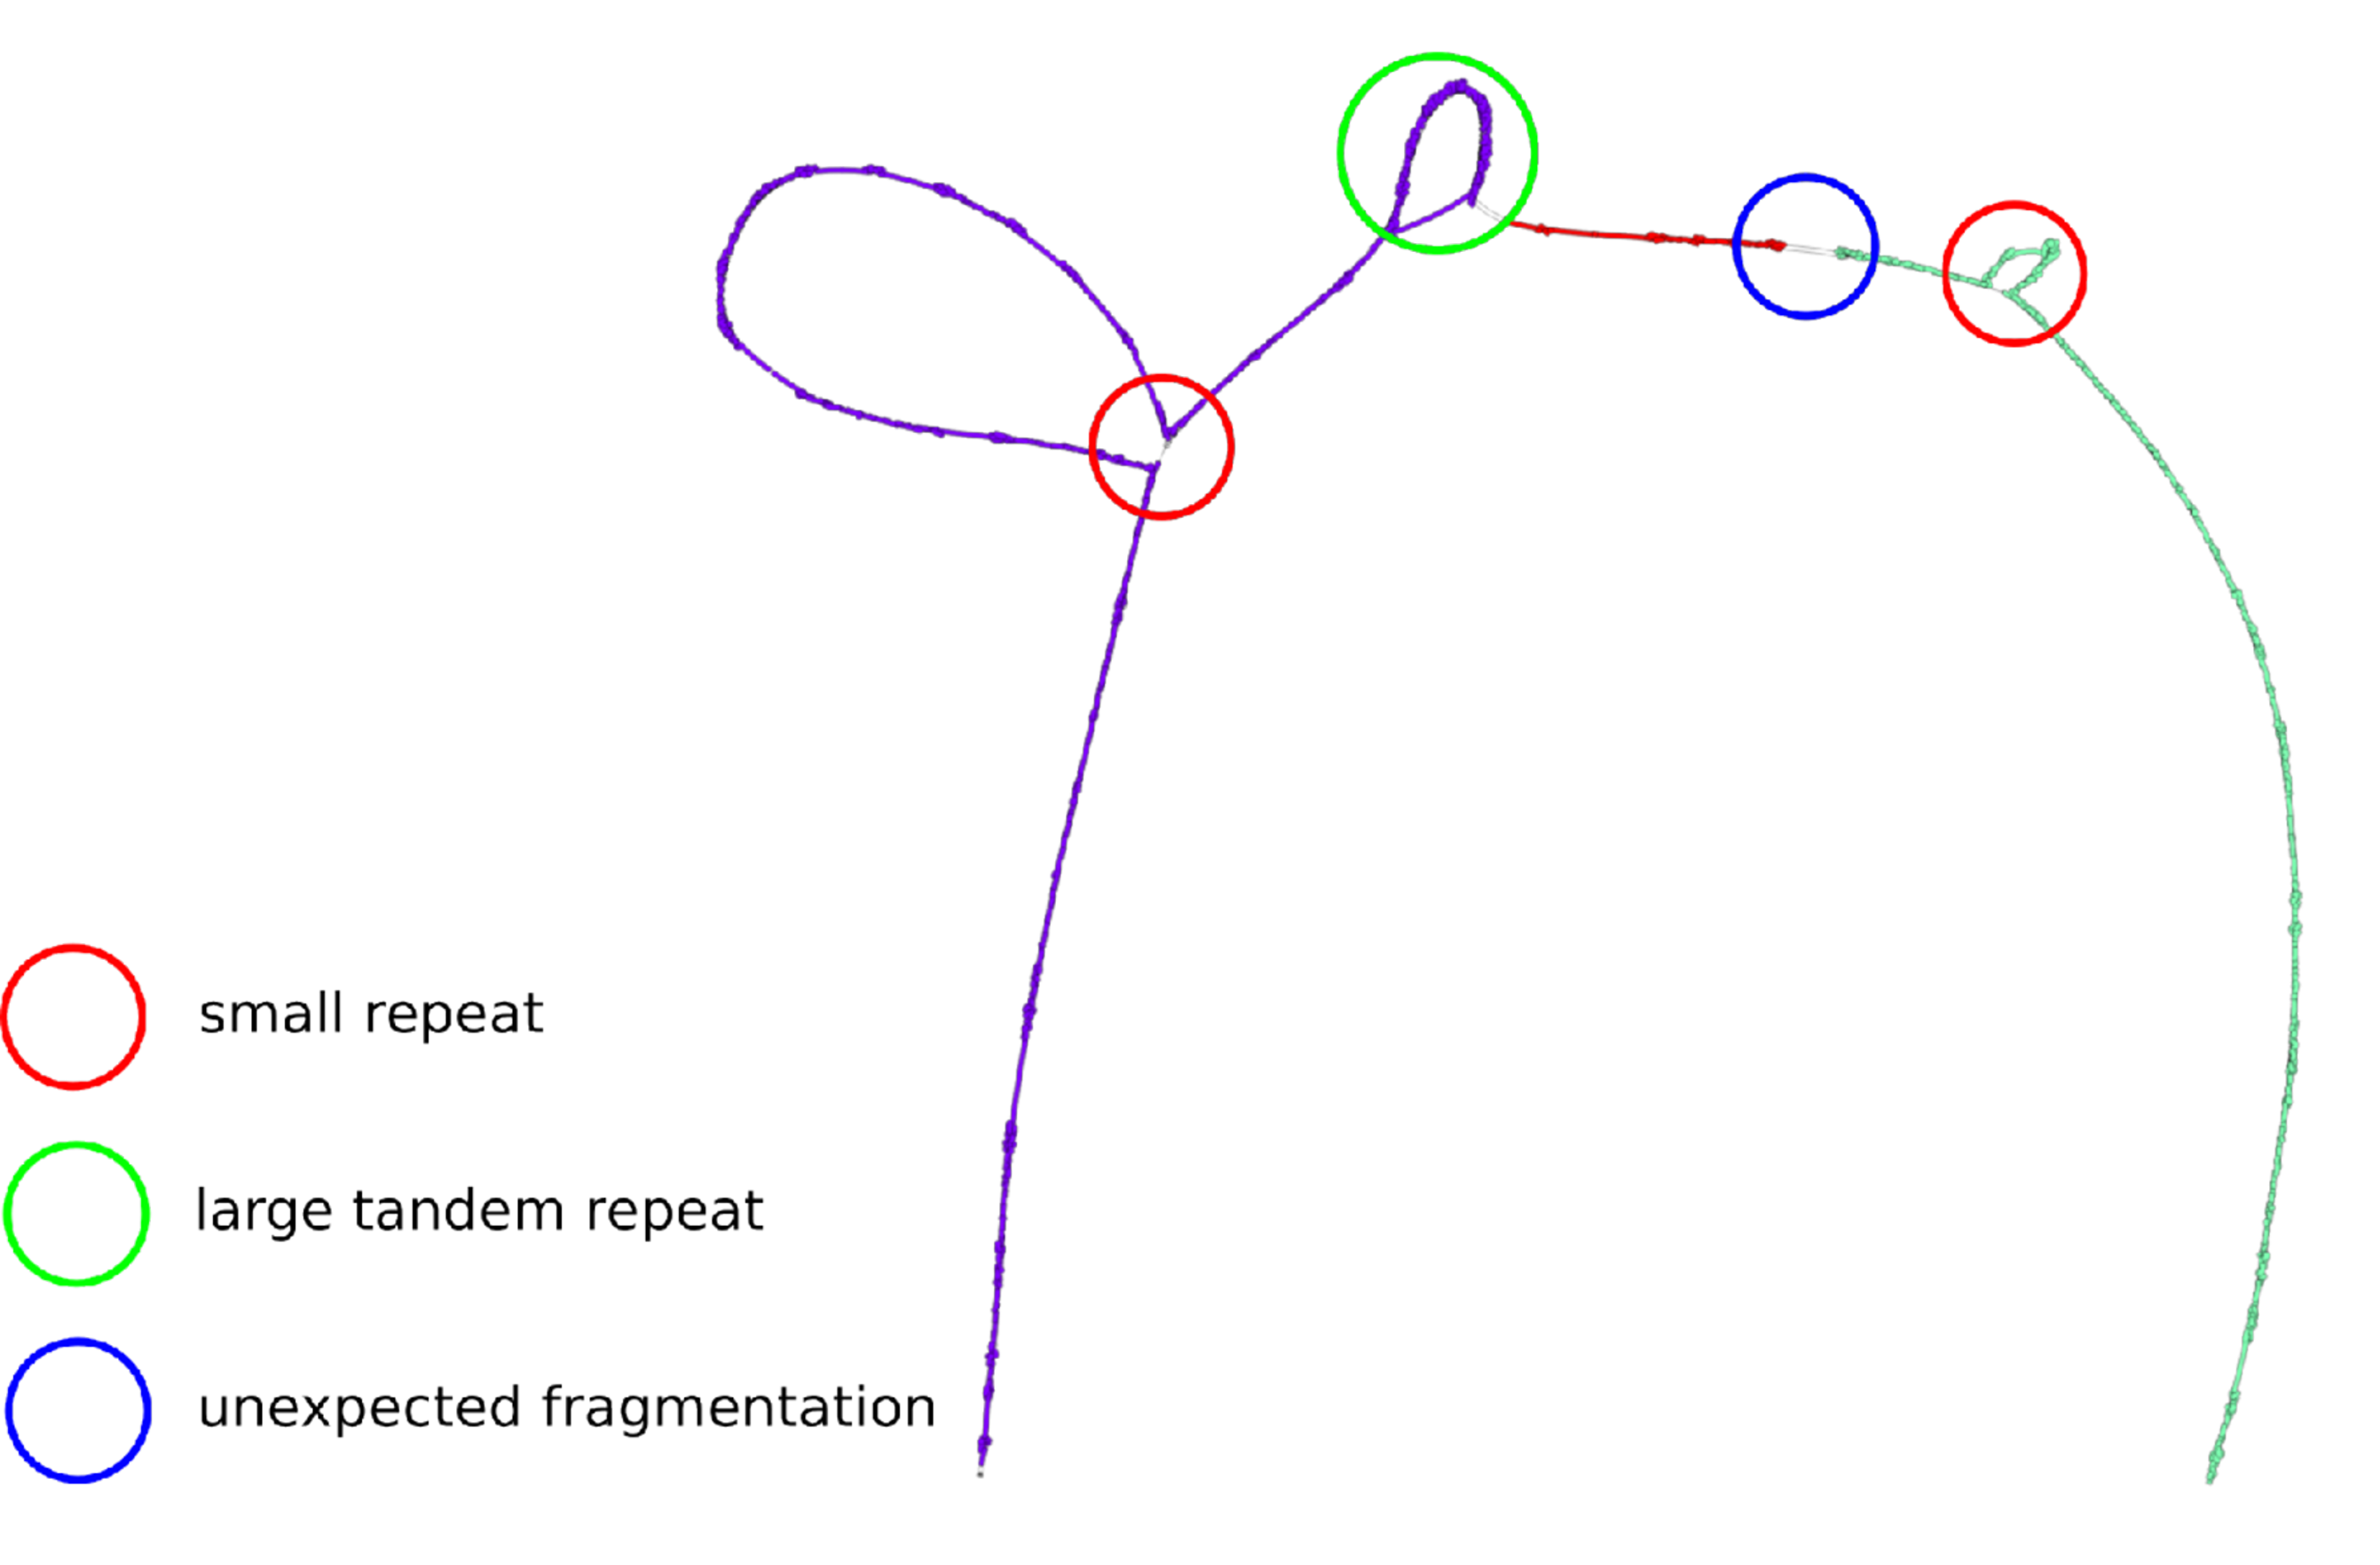
\includegraphics[width=\textwidth]{postassembly/images/t_roseus_projection_annoted.pdf}
    \caption{This graph is the overlap graph (computed by \minimap), reads used by \canu to build its contigs are colored with same color. We can observe two fragmentation points, one can be explained by a repetition, green circle, we can observe repetition solved by \canu, but the fragmentation between green and red can't be explain by a repetition.}%Plus simple pls
    \label{postassembly:fig:t_roseus_example}
\end{figure}

The Figure \ref{postassembly:fig:t_roseus_example} present the main idea of \knot, to combine information of assembly (the read coloration) with a maximum of information that can be extracted from reads (the \OLC graph build from \minimap but another overlapping tools can be used). The   contigs information help us to ignore some already solved problem (red circle), unsolvable trouble (greed circle) and  to focus on strange situations (blue circle). Figure \ref{postassembly:fig:t_roseus_example} show a very simple example on a real case. The \OLC graph can be unreadable. For these reason and to run analysis without an human intervention we also automatised the idea of \knot.%UNCLEAR

The paper was publish originally publish in Bioinformatics (\url{https://doi.org/10.1093/bioinformatics/btz219}), we reformat the paper in the style of this current document for reasons of readability.

\subfile{paper/knot.tex}

\section{Conclusion}

In this section we studied how we can evaluate an assembly, and detailed some issues when we use a reference genome to evaluate a de novo long-read assemblies.

With \knot we present the interest to go back to raw read information, and how it can solve  bacterial assembly issues.
To use \knot on more complex datasets we need improve some part of \knot, especially the graph construction, its representation in memory and the search of paths between contigs extremity. This improvements required some development, but the original idea of going back to raw reads information can be used for more genome assembly improvements. I present this idea in my conclusion. %on peux faire mieux comme phrase de fin de chapitre



\end{document}